\documentclass[twoside]{book}

% Packages required by doxygen
\usepackage{calc}
\usepackage{doxygen}
\usepackage{graphicx}
\usepackage[utf8]{inputenc}
\usepackage{makeidx}
\usepackage{multicol}
\usepackage{multirow}
\usepackage{textcomp}
\usepackage[table]{xcolor}

% Font selection
\usepackage[T1]{fontenc}
\usepackage{mathptmx}
\usepackage[scaled=.90]{helvet}
\usepackage{courier}
\usepackage{amssymb}
\usepackage{sectsty}
\renewcommand{\familydefault}{\sfdefault}
\allsectionsfont{%
  \fontseries{bc}\selectfont%
  \color{darkgray}%
}
\renewcommand{\DoxyLabelFont}{%
  \fontseries{bc}\selectfont%
  \color{darkgray}%
}

% Page & text layout
\usepackage{geometry}
\geometry{%
  a4paper,%
  top=2.5cm,%
  bottom=2.5cm,%
  left=2.5cm,%
  right=2.5cm%
}
\tolerance=750
\hfuzz=15pt
\hbadness=750
\setlength{\emergencystretch}{15pt}
\setlength{\parindent}{0cm}
\setlength{\parskip}{0.2cm}
\makeatletter
\renewcommand{\paragraph}{%
  \@startsection{paragraph}{4}{0ex}{-1.0ex}{1.0ex}{%
    \normalfont\normalsize\bfseries\SS@parafont%
  }%
}
\renewcommand{\subparagraph}{%
  \@startsection{subparagraph}{5}{0ex}{-1.0ex}{1.0ex}{%
    \normalfont\normalsize\bfseries\SS@subparafont%
  }%
}
\makeatother

% Headers & footers
\usepackage{fancyhdr}
\pagestyle{fancyplain}
\fancyhead[LE]{\fancyplain{}{\bfseries\thepage}}
\fancyhead[CE]{\fancyplain{}{}}
\fancyhead[RE]{\fancyplain{}{\bfseries\leftmark}}
\fancyhead[LO]{\fancyplain{}{\bfseries\rightmark}}
\fancyhead[CO]{\fancyplain{}{}}
\fancyhead[RO]{\fancyplain{}{\bfseries\thepage}}
\fancyfoot[LE]{\fancyplain{}{}}
\fancyfoot[CE]{\fancyplain{}{}}
\fancyfoot[RE]{\fancyplain{}{\bfseries\scriptsize Generated on Sun Mar 1 2015 19\-:58\-:32 for Crazy River Ride by Doxygen }}
\fancyfoot[LO]{\fancyplain{}{\bfseries\scriptsize Generated on Sun Mar 1 2015 19\-:58\-:32 for Crazy River Ride by Doxygen }}
\fancyfoot[CO]{\fancyplain{}{}}
\fancyfoot[RO]{\fancyplain{}{}}
\renewcommand{\footrulewidth}{0.4pt}
\renewcommand{\chaptermark}[1]{%
  \markboth{#1}{}%
}
\renewcommand{\sectionmark}[1]{%
  \markright{\thesection\ #1}%
}

% Indices & bibliography
\usepackage{natbib}
\usepackage[titles]{tocloft}
\setcounter{tocdepth}{3}
\setcounter{secnumdepth}{5}
\makeindex

% Hyperlinks (required, but should be loaded last)
\usepackage{ifpdf}
\ifpdf
  \usepackage[pdftex,pagebackref=true]{hyperref}
\else
  \usepackage[ps2pdf,pagebackref=true]{hyperref}
\fi
\hypersetup{%
  colorlinks=true,%
  linkcolor=blue,%
  citecolor=blue,%
  unicode%
}

% Custom commands
\newcommand{\clearemptydoublepage}{%
  \newpage{\pagestyle{empty}\cleardoublepage}%
}


%===== C O N T E N T S =====

\begin{document}

% Titlepage & ToC
\hypersetup{pageanchor=false}
\pagenumbering{roman}
\begin{titlepage}
\vspace*{7cm}
\begin{center}%
{\Large Crazy River Ride }\\
\vspace*{1cm}
{\large Generated by Doxygen 1.8.6}\\
\vspace*{0.5cm}
{\small Sun Mar 1 2015 19:58:32}\\
\end{center}
\end{titlepage}
\clearemptydoublepage
\tableofcontents
\clearemptydoublepage
\pagenumbering{arabic}
\hypersetup{pageanchor=true}

%--- Begin generated contents ---
\chapter{Hierarchical Index}
\section{Class Hierarchy}
This inheritance list is sorted roughly, but not completely, alphabetically\-:\begin{DoxyCompactList}
\item Observer\begin{DoxyCompactList}
\item \contentsline{section}{Game\-Manager}{\pageref{class_game_manager}}{}
\item \contentsline{section}{Key\-Updater}{\pageref{class_key_updater}}{}
\end{DoxyCompactList}
\item \contentsline{section}{Paint\-Task}{\pageref{class_paint_task}}{}
\item Q\-Main\-Window\begin{DoxyCompactList}
\item \contentsline{section}{Crazy\-River\-Ride}{\pageref{class_crazy_river_ride}}{}
\end{DoxyCompactList}
\item Q\-Thread\begin{DoxyCompactList}
\item \contentsline{section}{Updater}{\pageref{class_updater}}{}
\end{DoxyCompactList}
\end{DoxyCompactList}

\chapter{Class Index}
\section{Class List}
Here are the classes, structs, unions and interfaces with brief descriptions\-:\begin{DoxyCompactList}
\item\contentsline{section}{\hyperlink{class_amount_box}{Amount\-Box} \\*Esta clase es la que se encarga de dar municiones al personaje, es la caja que aparece aleatoriamente sobre la ventana y da las municiones o disparos }{\pageref{class_amount_box}}{}
\item\contentsline{section}{\hyperlink{class_angle_shot}{Angle\-Shot} }{\pageref{class_angle_shot}}{}
\item\contentsline{section}{\hyperlink{class_angle_shot_manager}{Angle\-Shot\-Manager} }{\pageref{class_angle_shot_manager}}{}
\item\contentsline{section}{\hyperlink{class_box}{Box} \\*Es la clase caja que se encarga de agregar puntos de vida al jugador, tambien se encarga de quitarle puntos si se ha convertido en una caja envenenada }{\pageref{class_box}}{}
\item\contentsline{section}{\hyperlink{class_bridge}{Bridge} }{\pageref{class_bridge}}{}
\item\contentsline{section}{\hyperlink{class_change_phase}{Change\-Phase} }{\pageref{class_change_phase}}{}
\item\contentsline{section}{\hyperlink{class_circular_list}{Circular\-List$<$ E $>$} \\*Esta clase es una estructura de datos especificamente una lista enlazada circular simple que puede contener cualquier tipo de dato solamente definiciendolo mediante el template de esta clase. se puede agregar y borrar el dato }{\pageref{class_circular_list}}{}
\item\contentsline{section}{\hyperlink{class_client_socket}{Client\-Socket} }{\pageref{class_client_socket}}{}
\item\contentsline{section}{\hyperlink{class_close}{Close} }{\pageref{class_close}}{}
\item\contentsline{section}{\hyperlink{class_combustible_box}{Combustible\-Box} \\*Es la caja que da combustible al jugador, o resta vida si el combustible ha sido consumido por los disparos del jugador(es) }{\pageref{class_combustible_box}}{}
\item\contentsline{section}{\hyperlink{class_comparer}{Comparer} }{\pageref{class_comparer}}{}
\item\contentsline{section}{\hyperlink{class_connection_manager}{Connection\-Manager} }{\pageref{class_connection_manager}}{}
\item\contentsline{section}{\hyperlink{class_control_player}{Control\-Player} }{\pageref{class_control_player}}{}
\item\contentsline{section}{\hyperlink{class_crazy_river_ride}{Crazy\-River\-Ride} }{\pageref{class_crazy_river_ride}}{}
\item\contentsline{section}{\hyperlink{class_crazy_thread}{Crazy\-Thread} \\*Clase superior no instanciable que representa a los thread del proyecto Crazy River Ride la implementacion de esta clase esta inspirada en la clase que se puede apreciar el en siguiente link }{\pageref{class_crazy_thread}}{}
\item\contentsline{section}{\hyperlink{class_create_player}{Create\-Player} }{\pageref{class_create_player}}{}
\item\contentsline{section}{\hyperlink{class_double_circular_list}{Double\-Circular\-List$<$ E $>$} \\*Esta clase es una estructura de datos especificamente una lista doblemente enlazada circular que puede contener cualquier tipo de dato solamente definiciendolo mediante el template de esta clase. se puede agregar y borrar el dato }{\pageref{class_double_circular_list}}{}
\item\contentsline{section}{\hyperlink{class_double_iterator}{Double\-Iterator$<$ E $>$} \\*Esta clase es un iterador de las listas doblemente enlazadas, ademas la actualizacion de la lista N\-O actualiza el iterador, por lo que el iterador es momentaneo. Es similar a una fotografia de una lista que no ha sido alterada si la lista se altera usando un iterador puede que el iterador falle. Por lo que es recomendable que la lista no se actualice mientras se usa un iterador }{\pageref{class_double_iterator}}{}
\item\contentsline{section}{\hyperlink{class_double_list}{Double\-List$<$ E $>$} \\*Esta clase es una estructura de datos especificamente una lista doblemente enlazada que puede contener cualquier tipo de dato solamente definiciendolo mediante el template de esta clase. se puede agregar y borrar el dato }{\pageref{class_double_list}}{}
\item\contentsline{section}{\hyperlink{class_double_list_adapter}{Double\-List\-Adapter$<$ E $>$} }{\pageref{class_double_list_adapter}}{}
\item\contentsline{section}{\hyperlink{class_double_node}{Double\-Node$<$ E $>$} \\*Es la parte elemental de una lista que sea doublemente enlazada }{\pageref{class_double_node}}{}
\item\contentsline{section}{\hyperlink{class_enemy_rocket}{Enemy\-Rocket} \\*Es la clase que filtra a las clases enemigo, es un clasificacion, pero aun asi es muy util como es el caso del uso del metodo shoot que lo implementa de tal forma que todos los enemigos los usen }{\pageref{class_enemy_rocket}}{}
\item\contentsline{section}{\hyperlink{class_game_loop}{Game\-Loop} \\*Es la clase que se encarga de controlar el pintado de la ventana del juego seccionandolo en frame por segundo, especificamente 24 fps, la clase regula el pintado y la ejecucion de las actualizaciones del juego mismo }{\pageref{class_game_loop}}{}
\item\contentsline{section}{\hyperlink{class_game_manager}{Game\-Manager} }{\pageref{class_game_manager}}{}
\item\contentsline{section}{\hyperlink{class_game_map}{Game\-Map} \\*Es el mapa del nivel }{\pageref{class_game_map}}{}
\item\contentsline{section}{\hyperlink{class_game_menu}{Game\-Menu} }{\pageref{class_game_menu}}{}
\item\contentsline{section}{\hyperlink{class_game_object}{Game\-Object} \\*Es el objeto principal del programa contiene todas las abstracciones posibles y pensadas por los programadores que trabajaron en ella. El objetivo de esta clase es abstraer la mayoria de las operaciones basicas y comunes entre objetos que contengan rectangulos y deban verificar si colisionan, no olvidando la caracteristica basica de los objetos de este juego,, la tendencia a estar en movimiento, a ser D\-I\-N\-A\-M\-I\-C\-O\-S. De esta clase derivan un monton, y son pocas en comparacion a su utilidad }{\pageref{class_game_object}}{}
\item\contentsline{section}{\hyperlink{class_game_object_notify}{Game\-Object\-Notify} }{\pageref{class_game_object_notify}}{}
\item\contentsline{section}{\hyperlink{class_gui_constanst}{Gui\-Constanst} }{\pageref{class_gui_constanst}}{}
\item\contentsline{section}{\hyperlink{class_h_p_entity}{H\-P\-Entity} \\*Es una derivacion de la clase \hyperlink{class_game_object}{Game\-Object}\} se encarga de estructurar aun mas el proyecto especializando algunos tipos de \hyperlink{class_game_object}{Game\-Object} y haciendo que estos tengan controles de vida, las clases que deriven de esta seran las que posean atributos de vida }{\pageref{class_h_p_entity}}{}
\item\contentsline{section}{\hyperlink{class_i_iterator}{I\-Iterator$<$ E $>$} \\*Es una interfaz para los iteradores hijos de este }{\pageref{class_i_iterator}}{}
\item\contentsline{section}{\hyperlink{class_i_list}{I\-List$<$ E $>$} \\*Es la interfaz de las listas }{\pageref{class_i_list}}{}
\item\contentsline{section}{\hyperlink{class_inverse_iterator}{Inverse\-Iterator$<$ E $>$} \\*Esta clase es un iterador de las listas doblemente enlazadas, ademas la actualizacion de la lista N\-O actualiza el iterador, por lo que el iterador es momentaneo. Es similar a una fotografia de una lista que no ha sido alterada si la lista se altera usando un iterador puede que el iterador falle. Por lo que es recomendable que la lista no se actualice mientras se usa un iterador. Ademas de que este iterador recorre la lista desde el dato final hasta el dato inicial }{\pageref{class_inverse_iterator}}{}
\item\contentsline{section}{\hyperlink{class_i_ordinate_list}{I\-Ordinate\-List$<$ E $>$} }{\pageref{class_i_ordinate_list}}{}
\item\contentsline{section}{\hyperlink{class_kamikaze}{Kamikaze} \\*La clase kamikaze representa a una nave detectora sige al jugador y detecta su posicion }{\pageref{class_kamikaze}}{}
\item\contentsline{section}{\hyperlink{class_kernel_game}{Kernel\-Game} }{\pageref{class_kernel_game}}{}
\item\contentsline{section}{\hyperlink{class_key_updater}{Key\-Updater} }{\pageref{class_key_updater}}{}
\item\contentsline{section}{\hyperlink{class_linear_shot}{Linear\-Shot} }{\pageref{class_linear_shot}}{}
\item\contentsline{section}{\hyperlink{class_linear_shot_fabric}{Linear\-Shot\-Fabric} }{\pageref{class_linear_shot_fabric}}{}
\item\contentsline{section}{\hyperlink{class_list}{List$<$ E $>$} \\*Esta clase es una estructura de datos especificamente una lista enlazada simple que puede contener cualquier tipo de dato solamente definiciendolo mediante el template de esta clase. se puede agregar y borrar el dato }{\pageref{class_list}}{}
\item\contentsline{section}{\hyperlink{class_mayhem_shot}{Mayhem\-Shot} }{\pageref{class_mayhem_shot}}{}
\item\contentsline{section}{\hyperlink{class_mayhem_shot_manager}{Mayhem\-Shot\-Manager} }{\pageref{class_mayhem_shot_manager}}{}
\item\contentsline{section}{\hyperlink{class_movil_enemy_rocket}{Movil\-Enemy\-Rocket} \\*Es un clase de nave enemiga que se mueve en linea recta y tambien horizontalmente }{\pageref{class_movil_enemy_rocket}}{}
\item\contentsline{section}{\hyperlink{class_node}{Node$<$ E $>$} \\*Es la parte elemental de una lista simple }{\pageref{class_node}}{}
\item\contentsline{section}{\hyperlink{class_observer}{Observer} \\*Es la clase que cumple con el patron de diseño observer Este es el observador al cual se le envian notificaciones y este las interpreta segun la implementacion de la clase hija que sobrescriba el metodo update de esta clase }{\pageref{class_observer}}{}
\item\contentsline{section}{\hyperlink{class_paint_task}{Paint\-Task} }{\pageref{class_paint_task}}{}
\item\contentsline{section}{\hyperlink{class_pause}{Pause} }{\pageref{class_pause}}{}
\item\contentsline{section}{\hyperlink{class_pause_other_players}{Pause\-Other\-Players} }{\pageref{class_pause_other_players}}{}
\item\contentsline{section}{\hyperlink{class_player}{Player} }{\pageref{class_player}}{}
\item\contentsline{section}{\hyperlink{class_player_is_created}{Player\-Is\-Created} }{\pageref{class_player_is_created}}{}
\item\contentsline{section}{\hyperlink{class_player_rocket}{Player\-Rocket} \\*Es la clase que representa la nave del jugador }{\pageref{class_player_rocket}}{}
\item\contentsline{section}{\hyperlink{class_player_status}{Player\-Status} }{\pageref{class_player_status}}{}
\item\contentsline{section}{\hyperlink{class_queue}{Queue$<$ E $>$} }{\pageref{class_queue}}{}
\item\contentsline{section}{\hyperlink{class_rocket}{Rocket} }{\pageref{class_rocket}}{}
\item\contentsline{section}{\hyperlink{class_select_map}{Select\-Map} }{\pageref{class_select_map}}{}
\item\contentsline{section}{\hyperlink{class_server_socket}{Server\-Socket} }{\pageref{class_server_socket}}{}
\item\contentsline{section}{\hyperlink{class_shot}{Shot} }{\pageref{class_shot}}{}
\item\contentsline{section}{\hyperlink{class_shot_fabric}{Shot\-Fabric} }{\pageref{class_shot_fabric}}{}
\item\contentsline{section}{\hyperlink{class_shot_manager}{Shot\-Manager} }{\pageref{class_shot_manager}}{}
\item\contentsline{section}{\hyperlink{class_simple_iterator}{Simple\-Iterator$<$ E $>$} \\*Esta clase es un iterador de las listas simples, ademas la actualizacion de la lista N\-O actualiza el iterador, por lo que el iterador es momentaneo. Es similar a una fotografia de una lista que no ha sido alterada si la lista se altera usando un iterador puede que el iterador falle. Por lo que es recomendable que la lista no se actualice mientras se usa un iterador }{\pageref{class_simple_iterator}}{}
\item\contentsline{section}{\hyperlink{class_simple_list_adapter}{Simple\-List\-Adapter$<$ E $>$} }{\pageref{class_simple_list_adapter}}{}
\item\contentsline{section}{\hyperlink{class_socket}{Socket} }{\pageref{class_socket}}{}
\item\contentsline{section}{\hyperlink{class_socket_exception}{Socket\-Exception} }{\pageref{class_socket_exception}}{}
\item\contentsline{section}{\hyperlink{class_stack}{Stack$<$ E $>$} }{\pageref{class_stack}}{}
\item\contentsline{section}{\hyperlink{struct_static_descriptor_initializer___change_phase__2eproto}{Static\-Descriptor\-Initializer\-\_\-\-Change\-Phase\-\_\-2eproto} }{\pageref{struct_static_descriptor_initializer___change_phase__2eproto}}{}
\item\contentsline{section}{\hyperlink{struct_static_descriptor_initializer___control_player__2eproto}{Static\-Descriptor\-Initializer\-\_\-\-Control\-Player\-\_\-2eproto} }{\pageref{struct_static_descriptor_initializer___control_player__2eproto}}{}
\item\contentsline{section}{\hyperlink{struct_static_descriptor_initializer___create_player__2eproto}{Static\-Descriptor\-Initializer\-\_\-\-Create\-Player\-\_\-2eproto} }{\pageref{struct_static_descriptor_initializer___create_player__2eproto}}{}
\item\contentsline{section}{\hyperlink{struct_static_descriptor_initializer___game_menu__2eproto}{Static\-Descriptor\-Initializer\-\_\-\-Game\-Menu\-\_\-2eproto} }{\pageref{struct_static_descriptor_initializer___game_menu__2eproto}}{}
\item\contentsline{section}{\hyperlink{struct_static_descriptor_initializer___game_object_notify__2eproto}{Static\-Descriptor\-Initializer\-\_\-\-Game\-Object\-Notify\-\_\-2eproto} }{\pageref{struct_static_descriptor_initializer___game_object_notify__2eproto}}{}
\item\contentsline{section}{\hyperlink{struct_static_descriptor_initializer___pause__2eproto}{Static\-Descriptor\-Initializer\-\_\-\-Pause\-\_\-2eproto} }{\pageref{struct_static_descriptor_initializer___pause__2eproto}}{}
\item\contentsline{section}{\hyperlink{struct_static_descriptor_initializer___pause_other_players__2eproto}{Static\-Descriptor\-Initializer\-\_\-\-Pause\-Other\-Players\-\_\-2eproto} }{\pageref{struct_static_descriptor_initializer___pause_other_players__2eproto}}{}
\item\contentsline{section}{\hyperlink{struct_static_descriptor_initializer___player_is_created__2eproto}{Static\-Descriptor\-Initializer\-\_\-\-Player\-Is\-Created\-\_\-2eproto} }{\pageref{struct_static_descriptor_initializer___player_is_created__2eproto}}{}
\item\contentsline{section}{\hyperlink{struct_static_descriptor_initializer___player_status__2eproto}{Static\-Descriptor\-Initializer\-\_\-\-Player\-Status\-\_\-2eproto} }{\pageref{struct_static_descriptor_initializer___player_status__2eproto}}{}
\item\contentsline{section}{\hyperlink{struct_static_descriptor_initializer___select_map__2eproto}{Static\-Descriptor\-Initializer\-\_\-\-Select\-Map\-\_\-2eproto} }{\pageref{struct_static_descriptor_initializer___select_map__2eproto}}{}
\item\contentsline{section}{\hyperlink{struct_static_descriptor_initializer___stop__2eproto}{Static\-Descriptor\-Initializer\-\_\-\-Stop\-\_\-2eproto} }{\pageref{struct_static_descriptor_initializer___stop__2eproto}}{}
\item\contentsline{section}{\hyperlink{class_subject}{Subject} \\*Es la clase \hyperlink{class_subject}{Subject} que se suscribe a un objeto de tipo observer y envia las notificaciones necesarias }{\pageref{class_subject}}{}
\item\contentsline{section}{\hyperlink{class_thread_helper}{Thread\-Helper} \\*Es un ayudante del \hyperlink{class_game_loop}{Game\-Loop}\} Este se comunica con la interfaz grafica del juego debido a que la ventana solo acepta objetos pertenecientes a qt y por ende esta clase hereda a Q\-Object }{\pageref{class_thread_helper}}{}
\item\contentsline{section}{\hyperlink{class_updater}{Updater} }{\pageref{class_updater}}{}
\end{DoxyCompactList}

\chapter{Class Documentation}
\hypertarget{class_crazy_river_ride}{\section{Crazy\-River\-Ride Class Reference}
\label{class_crazy_river_ride}\index{Crazy\-River\-Ride@{Crazy\-River\-Ride}}
}
Inheritance diagram for Crazy\-River\-Ride\-:\begin{figure}[H]
\begin{center}
\leavevmode
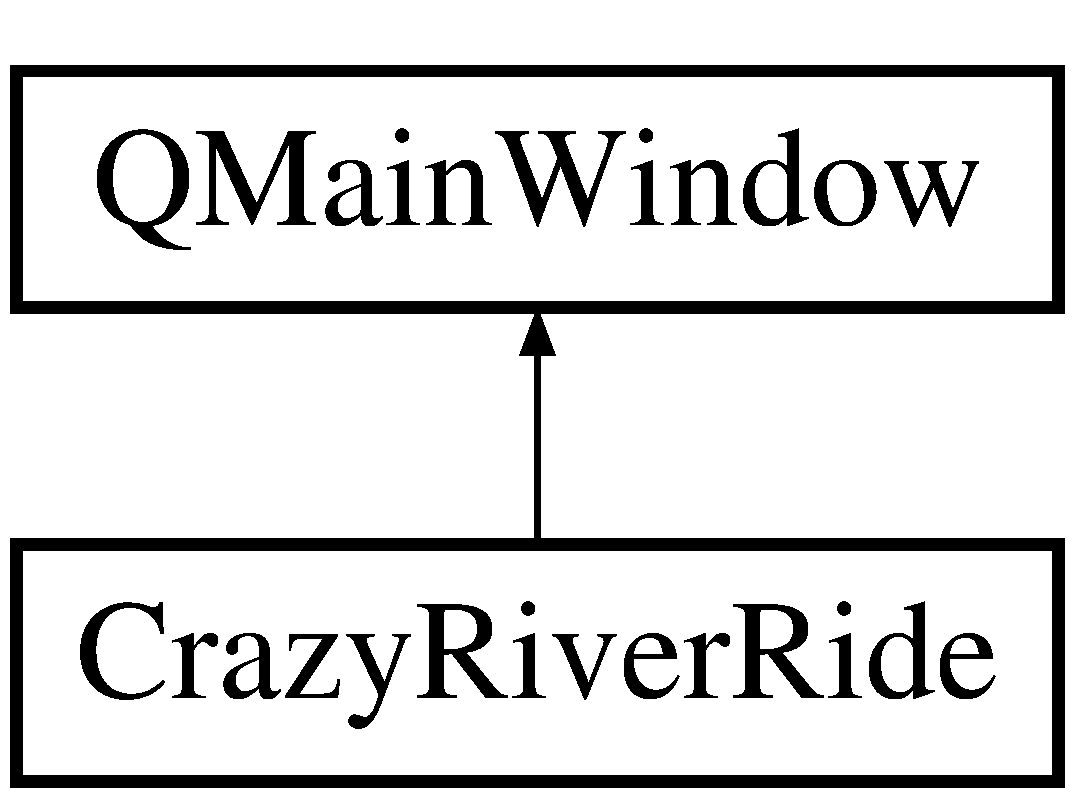
\includegraphics[height=2.000000cm]{class_crazy_river_ride}
\end{center}
\end{figure}
\subsection*{Public Slots}
\begin{DoxyCompactItemize}
\item 
\hypertarget{class_crazy_river_ride_a723a8b3355778a13d7d1e3a3e45d30a0}{void {\bfseries render} ()}\label{class_crazy_river_ride_a723a8b3355778a13d7d1e3a3e45d30a0}

\end{DoxyCompactItemize}
\subsection*{Public Member Functions}
\begin{DoxyCompactItemize}
\item 
\hypertarget{class_crazy_river_ride_ae7676b37caf1b9f9687eb1de0b426b77}{{\bfseries Crazy\-River\-Ride} (Q\-Widget $\ast$parent=0)}\label{class_crazy_river_ride_ae7676b37caf1b9f9687eb1de0b426b77}

\item 
\hypertarget{class_crazy_river_ride_a6f69c5acd7124489c8e95024debec646}{void {\bfseries paint\-Image} (Q\-Rect rec, Q\-Pixmap $\ast$p\-Image)}\label{class_crazy_river_ride_a6f69c5acd7124489c8e95024debec646}

\item 
\hypertarget{class_crazy_river_ride_a915fc6fab259b6fa24b09e64b7710e9c}{int {\bfseries get\-Key\-Xaxis} ()}\label{class_crazy_river_ride_a915fc6fab259b6fa24b09e64b7710e9c}

\item 
\hypertarget{class_crazy_river_ride_a175a99b902ffc945943acc281fb28165}{int {\bfseries get\-Key\-Yaxis} ()}\label{class_crazy_river_ride_a175a99b902ffc945943acc281fb28165}

\item 
\hypertarget{class_crazy_river_ride_ab19f0f54728bec4069aa4c20e547be3c}{bool {\bfseries is\-Running} ()}\label{class_crazy_river_ride_ab19f0f54728bec4069aa4c20e547be3c}

\item 
\hypertarget{class_crazy_river_ride_a25bba6ef360d73e9bd2b43157f0eea0f}{void {\bfseries setkey\-Updater} (\hyperlink{class_key_updater}{Key\-Updater} p\-Key\-Updater)}\label{class_crazy_river_ride_a25bba6ef360d73e9bd2b43157f0eea0f}

\item 
\hypertarget{class_crazy_river_ride_a8e04c2ebe8c0397fada83df2bd736a80}{int {\bfseries get\-Playerlife} () const }\label{class_crazy_river_ride_a8e04c2ebe8c0397fada83df2bd736a80}

\item 
\hypertarget{class_crazy_river_ride_a6314d065ea228fd3464d41989ea56d69}{void {\bfseries set\-Playerlife} (int value)}\label{class_crazy_river_ride_a6314d065ea228fd3464d41989ea56d69}

\item 
\hypertarget{class_crazy_river_ride_a5c94c18d81438b715178bf4d27db79ac}{int {\bfseries get\-Playerpoints} () const }\label{class_crazy_river_ride_a5c94c18d81438b715178bf4d27db79ac}

\item 
\hypertarget{class_crazy_river_ride_ae422c0571f910c124ed96c680892d19b}{void {\bfseries set\-Playerpoints} (int value)}\label{class_crazy_river_ride_ae422c0571f910c124ed96c680892d19b}

\item 
\hypertarget{class_crazy_river_ride_adab75d641f8df41b15851c0139b37cd3}{int {\bfseries get\-Playermunition} () const }\label{class_crazy_river_ride_adab75d641f8df41b15851c0139b37cd3}

\item 
\hypertarget{class_crazy_river_ride_ae773c56d054fd73adadf6f2ab3e725e1}{void {\bfseries set\-Playermunition} (int value)}\label{class_crazy_river_ride_ae773c56d054fd73adadf6f2ab3e725e1}

\item 
\hypertarget{class_crazy_river_ride_a33d1c49da5c75f486a5a6cf468ea194d}{void {\bfseries set\-Renderin\-Type} (bool is\-On\-Menu, bool is\-Game\-Over)}\label{class_crazy_river_ride_a33d1c49da5c75f486a5a6cf468ea194d}

\item 
\hypertarget{class_crazy_river_ride_a7ff417550948dd28d538e614fd23d91b}{int {\bfseries get\-Player\-Combustible} () const }\label{class_crazy_river_ride_a7ff417550948dd28d538e614fd23d91b}

\item 
\hypertarget{class_crazy_river_ride_ab9d581ecdc75251102d8c243d47fbe00}{void {\bfseries set\-Player\-Combustible} (int value)}\label{class_crazy_river_ride_ab9d581ecdc75251102d8c243d47fbe00}

\item 
\hypertarget{class_crazy_river_ride_a48c19baeb07b2e81d2663adc70ede714}{void {\bfseries playmusic} ()}\label{class_crazy_river_ride_a48c19baeb07b2e81d2663adc70ede714}

\end{DoxyCompactItemize}
\subsection*{Protected Member Functions}
\begin{DoxyCompactItemize}
\item 
\hypertarget{class_crazy_river_ride_a1b5346e20df6444e9cdd3e3c978d6a67}{void {\bfseries close\-Event} (Q\-Close\-Event $\ast$)}\label{class_crazy_river_ride_a1b5346e20df6444e9cdd3e3c978d6a67}

\item 
\hypertarget{class_crazy_river_ride_a8a163207bf92442bdfe0ea382d6e7e7d}{void {\bfseries paint\-Event} (Q\-Paint\-Event $\ast$)}\label{class_crazy_river_ride_a8a163207bf92442bdfe0ea382d6e7e7d}

\item 
\hypertarget{class_crazy_river_ride_a87f27420c335b9b693e7dcfe8e0c3281}{void {\bfseries key\-Press\-Event} (Q\-Key\-Event $\ast$)}\label{class_crazy_river_ride_a87f27420c335b9b693e7dcfe8e0c3281}

\item 
\hypertarget{class_crazy_river_ride_af0846544ef52af8e9f7476fa9f7f2f73}{void {\bfseries key\-Release\-Event} (Q\-Key\-Event $\ast$)}\label{class_crazy_river_ride_af0846544ef52af8e9f7476fa9f7f2f73}

\end{DoxyCompactItemize}


The documentation for this class was generated from the following files\-:\begin{DoxyCompactItemize}
\item 
crazyriverride.\-h\item 
crazyriverride.\-cpp\end{DoxyCompactItemize}

\hypertarget{class_game_manager}{\section{Game\-Manager Class Reference}
\label{class_game_manager}\index{Game\-Manager@{Game\-Manager}}
}
Inheritance diagram for Game\-Manager\-:\begin{figure}[H]
\begin{center}
\leavevmode
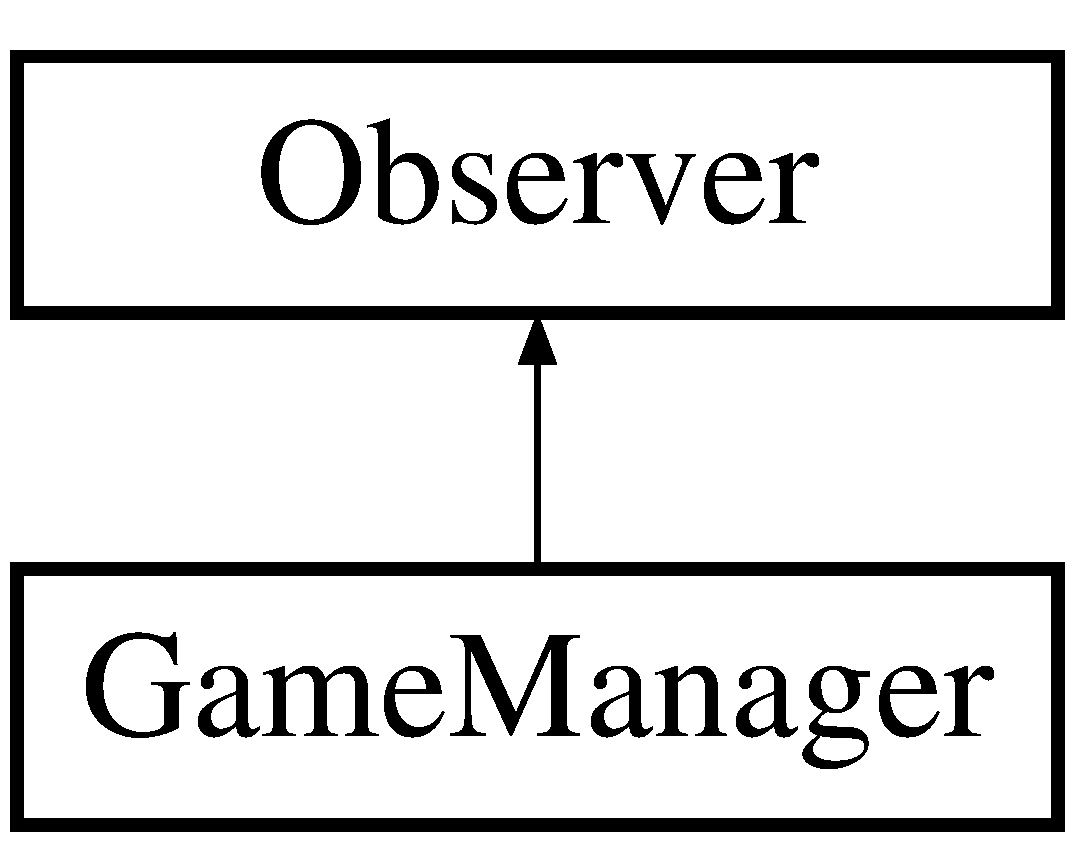
\includegraphics[height=2.000000cm]{class_game_manager}
\end{center}
\end{figure}
\subsection*{Public Member Functions}
\begin{DoxyCompactItemize}
\item 
\hypertarget{class_game_manager_a8ca3e8bfd80b9c5637a279ba0a779859}{{\bfseries Game\-Manager} (\hyperlink{class_crazy_river_ride}{Crazy\-River\-Ride} $\ast$)}\label{class_game_manager_a8ca3e8bfd80b9c5637a279ba0a779859}

\item 
\hypertarget{class_game_manager_a46f13cda874d5146c65db959d44607c8}{void {\bfseries run\-A\-Game} ()}\label{class_game_manager_a46f13cda874d5146c65db959d44607c8}

\item 
\hypertarget{class_game_manager_a24ac94e016dc0ad440faa7b88ee31840}{int {\bfseries get\-X\-Axis} ()}\label{class_game_manager_a24ac94e016dc0ad440faa7b88ee31840}

\item 
\hypertarget{class_game_manager_abe4ae648e6067c8bd19a1d020c292560}{int {\bfseries get\-Y\-Axis} ()}\label{class_game_manager_abe4ae648e6067c8bd19a1d020c292560}

\item 
\hypertarget{class_game_manager_a6b43e9e166a906789e4b4aa134218994}{bool {\bfseries shoot} ()}\label{class_game_manager_a6b43e9e166a906789e4b4aa134218994}

\item 
\hypertarget{class_game_manager_a91a7e823176e56f32ca0b582592d7b02}{bool {\bfseries pause} ()}\label{class_game_manager_a91a7e823176e56f32ca0b582592d7b02}

\item 
\hypertarget{class_game_manager_a0c03dfd4e0fd50e0d9159da2b3d15342}{void {\bfseries select} (int Map)}\label{class_game_manager_a0c03dfd4e0fd50e0d9159da2b3d15342}

\item 
void \hyperlink{class_game_manager_abcc7beda88f37957ab1c0711de030a45}{update} (google\-::protobuf\-::\-Message $\ast$p\-Message)
\begin{DoxyCompactList}\small\item\em Recibe un mensaje mediante el uso de protocol buffers de google Recibe el protocolo, y lo decodifica con la implementacion necesaria que se le de al la clase que sobrescriba este metodo virtual. \end{DoxyCompactList}\end{DoxyCompactItemize}


\subsection{Member Function Documentation}
\hypertarget{class_game_manager_abcc7beda88f37957ab1c0711de030a45}{\index{Game\-Manager@{Game\-Manager}!update@{update}}
\index{update@{update}!GameManager@{Game\-Manager}}
\subsubsection[{update}]{\setlength{\rightskip}{0pt plus 5cm}void Game\-Manager\-::update (
\begin{DoxyParamCaption}
\item[{google\-::protobuf\-::\-Message $\ast$}]{p\-Message}
\end{DoxyParamCaption}
)\hspace{0.3cm}{\ttfamily [virtual]}}}\label{class_game_manager_abcc7beda88f37957ab1c0711de030a45}


Recibe un mensaje mediante el uso de protocol buffers de google Recibe el protocolo, y lo decodifica con la implementacion necesaria que se le de al la clase que sobrescriba este metodo virtual. 


\begin{DoxyParams}{Parameters}
{\em p\-Message} & Es el mensaje recibido que es parte de los protocol buffers de google \\
\hline
\end{DoxyParams}


Implements \hyperlink{class_observer_a7204fd48ae9f9c2f39ea7e165740c451}{Observer}.



The documentation for this class was generated from the following files\-:\begin{DoxyCompactItemize}
\item 
gamemanager.\-h\item 
gamemanager.\-cpp\end{DoxyCompactItemize}

\hypertarget{class_key_updater}{\section{Key\-Updater Class Reference}
\label{class_key_updater}\index{Key\-Updater@{Key\-Updater}}
}
Inheritance diagram for Key\-Updater\-:\begin{figure}[H]
\begin{center}
\leavevmode
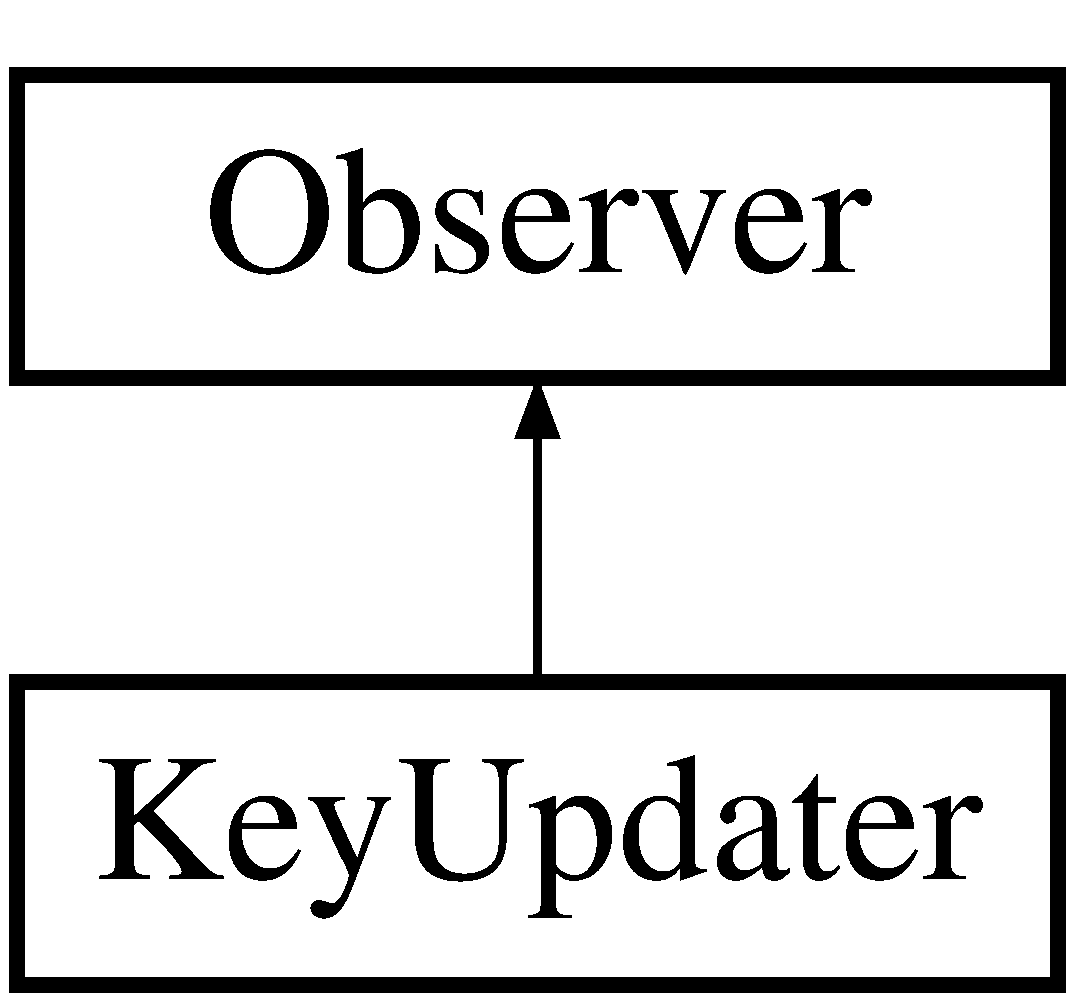
\includegraphics[height=2.000000cm]{class_key_updater}
\end{center}
\end{figure}
\subsection*{Public Member Functions}
\begin{DoxyCompactItemize}
\item 
\hypertarget{class_key_updater_a9e36344e5b6ea74cd35d64b00b108a18}{{\bfseries Key\-Updater} (Kernel\-Game $\ast$kg)}\label{class_key_updater_a9e36344e5b6ea74cd35d64b00b108a18}

\item 
\hypertarget{class_key_updater_ae98e44fb4a0be038fd6482bfae40007e}{void {\bfseries update} (google\-::protobuf\-::\-Message $\ast$p\-Message)}\label{class_key_updater_ae98e44fb4a0be038fd6482bfae40007e}

\end{DoxyCompactItemize}


The documentation for this class was generated from the following files\-:\begin{DoxyCompactItemize}
\item 
/home/cristianfernando/\-Documentos/git/\-Crazy\-River\-Ride/src/keyupdater.\-h\item 
/home/cristianfernando/\-Documentos/git/\-Crazy\-River\-Ride/src/keyupdater.\-cpp\end{DoxyCompactItemize}

\hypertarget{class_paint_task}{\section{Paint\-Task Class Reference}
\label{class_paint_task}\index{Paint\-Task@{Paint\-Task}}
}
\subsection*{Public Member Functions}
\begin{DoxyCompactItemize}
\item 
\hypertarget{class_paint_task_a95c518e8d1f1b47513fcbb7d33efae92}{{\bfseries Paint\-Task} (Q\-Rect p\-Rec, Q\-Pixmap $\ast$p\-Pix)}\label{class_paint_task_a95c518e8d1f1b47513fcbb7d33efae92}

\item 
\hypertarget{class_paint_task_aa6a868686cea358b91056a7bdd17c39c}{{\bfseries Paint\-Task} (const \hyperlink{class_paint_task}{Paint\-Task} \&pt)}\label{class_paint_task_aa6a868686cea358b91056a7bdd17c39c}

\item 
\hypertarget{class_paint_task_a2cfc517eefcaf5190c3c138402edf24a}{Q\-Rect {\bfseries get\-Rec} () const }\label{class_paint_task_a2cfc517eefcaf5190c3c138402edf24a}

\item 
\hypertarget{class_paint_task_a589af1cb82beb781e4cc34027f73bdf0}{void {\bfseries set\-Rec} (const Q\-Rect \&value)}\label{class_paint_task_a589af1cb82beb781e4cc34027f73bdf0}

\item 
\hypertarget{class_paint_task_ad32c94ebc7a9b5640179ccbf00a0398e}{Q\-Pixmap $\ast$ {\bfseries get\-Pix} () const }\label{class_paint_task_ad32c94ebc7a9b5640179ccbf00a0398e}

\item 
\hypertarget{class_paint_task_aba6f4430d04a3202950719145f89597c}{void {\bfseries set\-Pix} (Q\-Pixmap $\ast$value)}\label{class_paint_task_aba6f4430d04a3202950719145f89597c}

\end{DoxyCompactItemize}


The documentation for this class was generated from the following files\-:\begin{DoxyCompactItemize}
\item 
painttask.\-h\item 
painttask.\-cpp\end{DoxyCompactItemize}

\hypertarget{class_updater}{\section{Updater Class Reference}
\label{class_updater}\index{Updater@{Updater}}
}
Inheritance diagram for Updater\-:\begin{figure}[H]
\begin{center}
\leavevmode
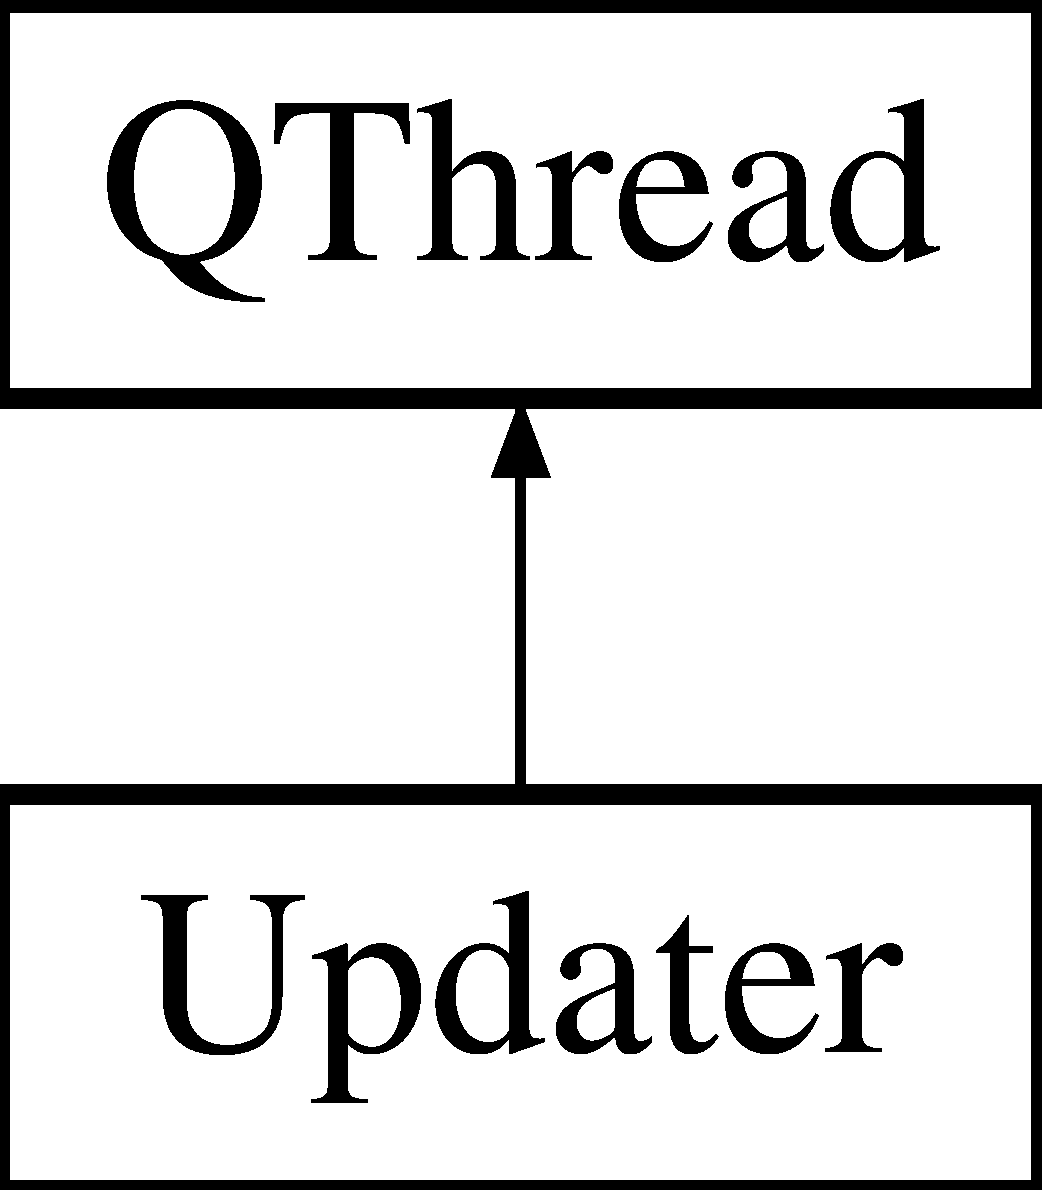
\includegraphics[height=2.000000cm]{class_updater}
\end{center}
\end{figure}
\subsection*{Signals}
\begin{DoxyCompactItemize}
\item 
\hypertarget{class_updater_aa443259cbce530ab39679cbe0220ad55}{void {\bfseries render\-Game} ()}\label{class_updater_aa443259cbce530ab39679cbe0220ad55}

\end{DoxyCompactItemize}
\subsection*{Public Member Functions}
\begin{DoxyCompactItemize}
\item 
\hypertarget{class_updater_adb60a473bc174de0ee06ee09c814e1a2}{{\bfseries Updater} (Q\-Object $\ast$parent=0)}\label{class_updater_adb60a473bc174de0ee06ee09c814e1a2}

\item 
\hypertarget{class_updater_a98324b20b804c73f2cb33fc01afd29fb}{void {\bfseries set\-Run\-Target} (Kernel\-Game $\ast$ogm)}\label{class_updater_a98324b20b804c73f2cb33fc01afd29fb}

\item 
\hypertarget{class_updater_abd76987a878910ff4687cac6cd63859d}{void {\bfseries run} ()}\label{class_updater_abd76987a878910ff4687cac6cd63859d}

\item 
\hypertarget{class_updater_aa115005ac2d83eead9c9ffd00a2faae7}{void {\bfseries set\-Active} (bool b)}\label{class_updater_aa115005ac2d83eead9c9ffd00a2faae7}

\item 
\hypertarget{class_updater_a055c8c65e3a0d7bd5af22f51f0541ba2}{bool {\bfseries is\-Close} ()}\label{class_updater_a055c8c65e3a0d7bd5af22f51f0541ba2}

\end{DoxyCompactItemize}


The documentation for this class was generated from the following files\-:\begin{DoxyCompactItemize}
\item 
/home/cristianfernando/\-Documentos/git/\-Crazy\-River\-Ride/src/updater.\-h\item 
/home/cristianfernando/\-Documentos/git/\-Crazy\-River\-Ride/src/updater.\-cpp\end{DoxyCompactItemize}

%--- End generated contents ---

% Index
\newpage
\phantomsection
\addcontentsline{toc}{chapter}{Index}
\printindex

\end{document}
